%\begin{savequote}[8cm]
%\textlatin{Cor animalium, fundamentum e\longs t vitæ, princeps omnium, Microco\longs mi Sol, a quo omnis vegetatio dependet, vigor omnis \& robur emanat.}
%
%The heart of animals is the foundation of their life, the sovereign of everything within them, the sun of their microcosm, that upon which all growth depends, from which all power proceeds.
%  \qauthor{--- William Harvey \cite{harvey_exercitatio_1628}}
%\end{savequote}

\chapter{\label{app:theory-ch4}Additional Theoretical Results For Chapter 4}


\htodo{Change N(s,m) to N(s,n) and then change N(s,n) to N to pow n of s.}

\todo{Currently a pasting ground for things cutting from theory section in Ch4 to make story not sound rubbish.}

\todo{Go through captions and make sure that we have short versions for all}



\section{The MCTS Stochastic Process}
\label{appsec:mcts_stoch_process}

    \todo{Words about how this is a lengthier version of the notation and preliminaries section? Make this section consistent with that section too}

    \todo{<beg> In main prose, but edited heavily. Keep some amount of this? Definitely keep the T and N stuff.}

        \todo{change m to n, and use mth when need to reason about prev trials (whole subsection)}

        When reasoning about a \textit{MCTS stochastic process} the following notations will be helpful.
        \begin{itemize}
            \item 
                The search policy used on the $m$th trial is $\pi^m$, and if the process were stopped after $m$ trials, the recommendation policy that the algorithm would output is denoted $\psi^m$. Where if the process is run for $n$ trials, then $m$ ranges from $1$ to $n$.
            \item 
                The $m$ trajectory sampled is $\tau^m=(s_0^m,a_0^m,...,s_{h-1}^m,a_{h-1}^m,s_{h}^m)$ \todo{add reward, also make it h subscript m instead of h?}, and is sampled using the search policy $\tau^m \sim \pi^m$ (that is $a^m_i \sim \pi^m(\cdot|s^m_i)$ and $s^m_{i+1} \sim p(\cdot | s^m_i, a^m_i)$). \todo{comment that $k$th trial is run until h where s subscript h is termal in some thtspp sense. Comment about how the superscripts on s a and r will be used when necessary, but not always}
            \item 
                The search tree after $m$ trials is denoted $\cl{T}^m$, the initial search tree is $\cl{T}^0=\{s_0\}$, and $\cl{T}^k = \cl{T}^{k-1} \cup \tau^k$.
        \end{itemize}

        When making arguments that apply to multiple algorithms the general policies $\pi$ and $\psi$ will be used, and when making arguments about specific algorithms the subscripts will be used, such as $\pibts$. Note that superscript is used to index with respect to the trial, and superscript with parenthasis is used to denote the number of visits.

        In the proofs of following sections, it will be useful to write the number of times state~$s$ was visited in the first $m$ trials as $N(s,m)$, and the number of times action~$a$ was selected from state~$s$ in the first m trials as $N(s,a,m).$ Additionally, it will be useful to write these quantities in terms of indicator random variables. 

        Let $T(s_t,m)$ (and $T(s_t,a_t,m)$) be the set of trajectory indices that $s_t$ was visited on (and action $a_t$ selected) in the first $m$ trials, that is: \todo{this can avoid using s subscript t}
        %
        \begin{align}
            T(s_t,m) &= \{i | i\leq m, s^i_t = s_t \} \\
            T(s_t,a_t,m) &= \{i | i\leq m, s^i_t = s_t, a^i_t = a_t \}.
        \end{align}
        %
        This allows the counts $N^m(s_t),$ $N^m(s_t,a_t)$ and $N^m(s_{t+1})$ (with $s_{t+1}\in\suc{s_t}{a_t}$) to be written as sums of indicator random variables in the following ways:
        %
        \begin{align}
            N(s_t,m) &= \sum_{i=1}^m \one[s^i_t=s_t] = |T(s_t,m)|, \\
            N(s_t,a_t,m) &= \sum_{i=1}^m \one[s^i_t=s_t,a^i_t=a_t] = |T(s_t,a_t,m)|, \\ 
            N(s_t,a_t,m) &= \sum_{i\in T(s_t,m)} \one[a^i_t = a_t], \label{appeq:nsa_sum} \\
            N(s_{t+1},m) &= \sum_{i\in T(s_t,a_t,m)} \one[s^i_{t+1} = s_{t+1}]. \label{appeq:ns_sum}
        \end{align}
        %
        Additionally, the assumption that for any two states $s,s'\in\cl{S}$ that $s=s'$ if and only if the trajectories leading to them are identical is made. This assumption is purely to simplify notation, so that nodes in the tree have a one-to-one correspondence with states (or state-action pairs). \todo{move this up}


    \todo{<end> In main prose, but edited heavily. Keep some amount of this?}



    \todo{do we do anything at all with the UCT process?}
    \todo{Maybe just write it out for completeness}

    \todo{Also add the backups for the number of visit function N into the backups in the full definitions in the appendices.}

    \todo{Also add the updates to the search tree. (Union of search tree with the trials.)}

    \todo{Handle setting the value at the end of the trial to Vinit in these processes too}

    \subsection{The UCT process.} 
    	The UCT search policy can be defined as:
        %
        \begin{align}
            \pi_{\textnormal{UCT}}^n(s_t) &= \max_{a\in\cl{A}} \text{UCB}^n(s_t,a), \\
            \text{UCB}^n(s_t, a) &= 
                    \begin{cases}
                        \infty & \text{if } N(s_t,a)=0 \\
                        \bar{Q}^{N(s_t,a)}(s_t, a)+c \sqrt{\frac{\log N(s_t)}{N(s_t, a)}} & \text{if } N(s_t,a)>0
                    \end{cases}
        \end{align}
        %
        \noindent where, after $n$ trials, $\bar{Q}^{N(s,a)}(s,a)$ is the empirical estimate of the value at node $(s,a)$, where action~$a$ has been selected $N(s, a)$ from state~$s$. The backup consists of updating empirical estimates for $t=h-1,...,0$:
        %
        \begin{align}
            \bar{V}^{N(s_t)+1}(s_t) &= \bar{V}^{N(s_t)}(s_t) + \frac{\bar{R}(t) - \bar{V}^{N(s_t)}(s_t)}{N(s_t) + 1}, \label{appeq:uct_vbar} \\
            \bar{Q}^{N(s_t,a_t)+1}(s_t, a_t) &= \bar{Q}^{N(s_t,a_t)}(s_t, a_t) + \frac{\bar{R}(t) - \bar{Q}^{N(s_t,a_t)}(s_t, a_t)}{N(s_t, a_t) + 1}, \label{appeq:uct_qbar}
        \end{align}
        %
        \noindent where $\bar{R}(t) = V^{\text{init}}(s_h) + \sum_{i=t}^{h-1} R(s_i,a_i)$, and values are initialised as $\bar{V}^1(s)=V^{\text{init}}(s)$ and $\bar{Q}^0(s,a)=0$. 
    

    
    
    
    \subsection{The MENTS Process}
    
        Below is a complete summary of the MENTS process, for reference. On the $m$th trial, the MENTS process follows the search policy:

        \todo{make ments section in ch2 use consistent definitions of alphaments, lambdaments and so on}

        \begin{align}
            \mpiments{m}(a|s) &= (1-\mlambdaments{m})\mrhoments{m}(a|s) + \frac{\mlambdaments{m}}{|\cl{A}|}, 
                        \label{appeq:ments_soft_policy} \\ 
            \mrhoments{m}(a|s) &= \exp\left(
                \frac{1}{\alphaments}\left(\mQments{N(s,a,m-1)}(s,a)-\mVments{N(s,m-1)}(s)\right)\right). \\
            \lambda^m(s,x) &= \min\left(1, \frac{x}{\log(e+N(s,m-1))}\right),
        \end{align}
        %
        where $\epsments\in(0,\infty)$ is an exploration parameters, and $\alphaments$ is the temperature parameter. 

        The $m$th trajectory is sampled using the search policy: $\tau^m \sim \piments^m$. Letting $\tau^m=(s_0,a_0,r_0,...,s_{h-1},a_{h-1},r_{h-1},s_{h})$, the MENTS value estimates are computed using backups for $t=h-1, ..., 0$: \todo{either add the superscript m into every s and a, or update words to say implicit}
        \begin{align}
            \mVments{N(s_t,m)}(s_t) &= 
                \alphaments \log \sum_{a\in\cl{A}} \exp \left(
                    \frac{1}{\alphaments}\mQments{N(s_t,a,m)}(s_t,a) \right), \label{appeq:soft_v_backup} \\
            \mQments{N(s_t,a_t,m)}(s_t,a_t) &= 
                R(s_t,a_t) + \sum_{s'\in\suc{s}{a}} \left( 
                    \frac{N(s',m)}{N(s_t,a_t,m)} \mVments{N(s',m)}(s') \right). \label{appeq:soft_q_backup}
        \end{align}

        \todo{also want something about initialisation and everything in line with thtspp}
        %
        % The soft (Q-)values are initialised as $\Vst{s}{1}=V^{\text{init}}(s)$ and $\Qst{s}{a}{0}=Q^{\text{init}}_{\sft}(s)$ (typically $Q^{\text{init}}_{\sft}(s)=0$).

        \todo{recommendation policies and some comment about it being the soft values used?}
        \begin{align}
            \mpsiments{m}(s) &= \argmax_{a\in\cl{A}}\mQments{N(s,a,m)}(s,a), \\
            \mmvments{m}(s) &= \argmax_{a\in\cl{A}} N(s,a,m).
        \end{align}





    \subsection{The DENTS Process}

        \todo{this whole sections math is pretty mess and a struggle to fit onto one line at a time. Maybe it suffices to just wordily describe the values of the sufixed values?}

        Follow policy: 
        %
        \todo{add more wordy things. Some things we said here before were: (1) defining beta} $\beta : \bb{R}\rightarrow [0,\infty)$ be a bounded function; \todo{(2) defined epsilon as exploration policy; (3) in Neurips we defined the propto version of rho and also the full version saying ``becasue we need to reason about the search policy we give the exact form,'' for the moment I've kept both. I think just copy the full version where relevent in the proofs.}
        %
        \begin{align}
            \mpidents{m}(a|s) &= (1-\mlambdadents{m})\mrhodents{m}(a|s) + \frac{\mlambdadents{m}}{|\cl{A}|}, 
                \label{appeq:dents_search_policy}  \\
            \mrhodents{m}(a|s) &\propto \exp\left(\frac{1}{\alphadents(N(s,m))}
                \left(\mQdents{N(s,a,m-1)}(s,a) + \betadents(N(s,m))\mHQdents{N(s,a,m-1)}(s,a) \right)\right). \\
            \mrhodents{m}(a|s) &= \frac{
                \exp\left(\frac{1}{\alphadents(N(s,m))}\left(
                    \mQdents{N(s,a,m-1)}(s,a) + \betadents(N(s,m))\mHQdents{N(s,a,m-1)}(s,a)   \right)\right)
                }{\sum\limits_{a'\in\cl{A}} \exp\left(\frac{1}{\alphadents(N(s,m))}\left(
                    \mQdents{N(s,a',m-1)}(s,a') + \betadents(N(s,m))\mHQdents{N(s,a',m-1)}(s,a')  \right)\right)}.  
                \label{appeq:full_rho} \\
            \lambda^m(s,x) &= \min\left(1, \frac{x}{\log(e+N(s,m-1))}\right), 
        \end{align}

        The $m$th trajectory is sampled using the search policy: $\tau^m \sim \pidents^m$. Letting $\tau^m=(s_0,a_0,r_0,...,s_{h-1},a_{h-1},r_{h-1},s_{h})$, the DENTS value and entropy estimates are computed using backups for $t=h-1, ..., 0$: \todo{either add the superscript m into every s and a, or update words to say implicit}
        \begin{align}
            \mQdents{N(s_t,a_t,m)}(s_t,a_t) &= 
                R(s_t,a_t) + \sum_{s' \in \suc{s_t}{a_t}} \left( 
                    \frac{N(s',m)}{N(s_t,a_t,m)} \mVdents{N(s',m)}(s') \right), 
                \label{appeq:dp_q_backup} \\ 
            \mVdents{N(s_t,m)}(s_t) &=\max_{a\in\cl{A}} \mQdents{N(s_t,a,m)}(s_t,a), 
                \label{appeq:dp_v_backup} \\
            \mHQdents{N(s_t,a_t,m)}(s_t,a_t) &= 
                \sum_{s'\in \suc{s_t}{a_t}} \frac{N(s',m)}{N(s_t,a_t,m)} \mHVdents{N(s',m)}(s'), \\
            \mHVdents{N(s_t)}(s_t) &= 
                \cl{H}(\mpidents{m}(\cdot | s_t)) 
                    + \sum_{a\in\cl{A}} \mpidents{m}(a_t|s_t)\mHQdents{N(s_t,a_t,m)}(s_t,a_t).
        \end{align}

        \todo{also want something about initialisation and everything in line with thtspp}
        %
        % The (Q-)values are initialised as $\Vt{s}{1}=V^{\text{init}}(s)$ and $\Qt{s}{a}{0}=Q^{\text{init}}_{\sft}(s)$ (typically $Q^{\text{init}}_{\sft}(s)=0$). The entropy values are initialised as $\cl{H}_Q^{0}(s,a)=0$ and $\cl{H}_V^{1}(s) = \cl{H}(\pi^n_{\text{DENTS}}(\cdot | s_t))$, where the node for $s$ is created on the $n$th trial

        \todo{recommendation policies word stuff}
        \begin{align}
            \mpsidents{m}(s) &= \argmax_{a\in\cl{A}}\mQdents{N(s,a,m)}(s,a), \\
            \mmvdents{m}(s) &= \argmax_{a\in\cl{A}} N(s,a,m).
        \end{align}

        \todo{From the neurips, also wrote the following (everything left in this subsubsection is copied and cleaned up, but probably needs a proof read)} Let $\mVrhodents{N(s)}(s)$ be defined as the value:
        %
        \begin{align}
            \mVrhodents{N(s)}(s) = &
                \alphadents(N(s,m)) \log \Bigg[ \sum_{a'\in\cl{A}} \exp\bigg(\frac{1}{\alphadents(N(s,m))}
                    \big(\mQdents{N(s,a')}(s,a') \nonumber \\
                &+ \betadents(N(s,m))\mHQdents{N(s,a')}(s,a') \big)\bigg)\Bigg], \label{appeq:v_rho}
        \end{align} 
        %
        and notice that the value of $\exp(\mVrhodents{N(s,m)}(s)/\alphadents(N(s,m)))$ is equal to the denominator in Equation (\ref{appeq:full_rho}), and so by rearranging we can write $\mrhodents{m}$ as 
        %
        \begin{align}
            \mrhodents{m}(a|s) = 
                \exp\left(\frac{1}{\alphadents(N(s,m))}\left(
                    \mQdents{N(s,a,m)}(s,a) 
                    + \betadents(N(s,m))\mHQdents{N(s,a,m)}(s,a) 
                    - \mVrhodents{N(s,m)}(s) \right)\right), \label{appeq:rho_concise}
        \end{align}
        % 
        and subsequently, the full DENTS policy can be written as:
        \begin{align}
            \mpidents{m}(a|s) = (1-\lambda(s,m))\exp\left(\frac{1}{\alphadents(N(s,m))}\left(\mQdents{N(s,a,m)}(s,a) + \betadents(N(s,m))\mHQdents{N(s,a)}(s,a) - \mVrhodents{N(s)}(s) \right)\right) + \frac{\lambda(s,m)}{|\cl{A}|}. \label{appeq:dents_search_policy_exact} 
        \end{align}








    \subsection{The AR-DENTS Process}
            
        \todo{Copy DENTS after its written. Swap out notation and backups.}








    \subsection{The (AR-)BTS process.}

        The (AR-)BTS process is a special case of the (AR-)DENTS process when $\betadents(x)=0$. As such, results about BTS will be corollaries from proofs about the (AR-)DENTS process.
















































\section{Exponential Convergence Results}
\label{appsec:exp}


    \todo{This section give proofs for exponential convergence results for DENTS and MENTS}, it is structured as follows:
    \begin{enumerate}
        \item First, Appendix \ref{appsec:exp-prelim} provides a set of Lemmas that are used later in the proofs for exponential convergence bounds;
        \item Second, Appendix \ref{appsec:max_entropy_results} gives Lemmas that provide sufficient conditions for the maximum entropy objective and standard objective to be aligned;
        \item Third, in Appendix \ref{appsec:q_result} it is shown in a general way that is Q-values are computed as a sample average of child value functions, and those child value functions admit a concentration inequality, then the Q-value also admits a concentration inequality;
        \item Fourth, in Appendix \ref{appsec:ments_results}, exponential convergence bounds (requiring restrictive conditions on the temperature parameter) are shown for MENTS; 
        \item Finally, in Appendix \ref{appsec:dents_proofs}, Theorem \ref{thrm:4:bts_exp} and \ref{thrm:4:dents_exp} are 
    \end{enumerate}

    \todo{Make sure that }

    \todo{Make sure assumptions and conditions stated. Anything that depends on the min prob needs to have the lower/upper bounds on the decay functions for example.}


    \subsection{Preliminaries}
    \label{appsec:exp-prelim}

        This subsection contains preliminary lemmas that are used for the building blocks to prove.
        
        \todo{<beg> dump}




            \todo{This section contains things related to exponential bounds, which might move to appendix}
            This subsection contains lemmas that will be useful in multiple times and are used to avoid repeating the same argument multiple times. 

            
            \todo{change m to n, and use mth when need to reason about prev trials (whole subsection)}





            Firstly it will be that the union of exponentially unlikely events is also exponentially unlikely, and that the intersection of exponentially likely events is exponentially likely. Although this is a special case of the union bound \todo{ref?} \todo{it is stated here so that it can be referenced, because this fact is used regularly }
            %
            \todo{Some comment about how this is just a special case of the union bound (and ref that?) and also }
            %
            \begin{lemma} \label{lem:union_bound}
                Let $A_1,...,A_{\ell}$ be some events that satisfy for $1\leq i \leq \ell$ the inequality $\Pr(\lnot A_i) \leq C_i\exp(-k_i)$ then:
                \begin{align}
                    \Pr\left(\bigcup_{i=1}^\ell \lnot A_i\right) &\leq C\exp(-k), \label{appeq:comb_exp_like} \\
                    \Pr\left(\bigcap_{i=1}^\ell A_i\right) = 1-\Pr\left(\bigcup_{i=1}^\ell \lnot A_i\right) &\geq 1-C\exp(-k), \label{appeq:exp_likely}
                \end{align}
                where $C=\sum_{i=1}^\ell C_i$ and $k = \min_i k_i$.
            \end{lemma}
            \begin{proofoutline}
                Lemma \ref{lem:union_bound} is a consequence of the union bound, using $\exp(k_i)\leq\exp(k)$ and simplifying. Inequality (\ref{appeq:exp_likely}) is just a negation of Inequality (\ref{appeq:comb_exp_like}).
            \end{proofoutline}






            
            The following two lemma's show that the MENTS and DENTS processes always have a minimum probability of picking any action. \todo{not in good headspace writing up these two lemmas. Do a clean up, double checking maths and that have eliminated using 'we' and so on}
            %
            \begin{lemma} \label{lem:min_prob_ments}
                For any MENTS process there exists some $\pi^{\min}>0$, for any state $s_t\in\cl{S}$, for all $a_t\in\cl{A}$ and any number of trials $m\in\bb{N}$, such that $\mpiments{m}(a_t|s_t)\geq\pi^{\min}$.
            \end{lemma}
            %
            \begin{proofoutline}
                \todo{Fix N having to be N(s,m) not N(s) etc}
                Define the $Q^{\min}$ function as follows:
                \begin{align}
                    Q^{\min}(s_t,a_t) = \min_{s_{t+1},a_{t+1},...,s_H,a_H} \sum_{i=t}^H \min(0, Q^{\text{init}}_{\sft}(s_i), R(s_i,a_i)).
                \end{align}
                \todo{clean up with respect to init function}
                
                And define the $V^{\max}$ function as:
                \begin{align}
                    V^{\max}(s_t) &= \alphaments \log \sum_{a\in\cl{A}} \exp (Q^{\max}(s_t,a)/\alphaments), \label{appeq:vmax} \\
                    Q^{\max}(s_t,a_t) &= R(s_t,a_t)+\max_{s_{t+1}\in\suc{s_t}{a_t}} V^{\max}(s_{t+1}).
                \end{align}
                
                Via induction, it is possible to show that $Q^{\min}(s_t,a_t)\leq \mQments{N(s_t,a_t,m)}(s_t,a_t)$ and $V^{\max}(s_t)\geq \mVments{N(s_t,m)}(s_t)$ for any arbitrary $s_t,a_t$ and $m$. Now, define $\pi^{\min}$ as:
                \begin{align}
                    \pi^{\min} = \inf_{\lambda\in[0,1]} \min_{(s,a)\in\cl{S}\times\cl{A}} (1-\lambda) \exp\left(\left(Q^{\min}(s,a)-V^{\max}(s)\right)/\alpha\right) + \frac{\lambda}{|\cl{A}|}. \label{eq:pi_min}
                \end{align}
                
                Because the value of an exponential is positive, as is $1/|\cl{A}|$, it follows that $\pi^{\min}>0.$ Recall the MENTS policy (Equation (\ref{appeq:ments_soft_policy})). By the monotonicity of the exponential function, it follows that for any $s_t\in\cl{S}, a_t\in\cl{A}, n\in\bb{N}$:
                \begin{align}
                    \mpiments{m}(a_t|s_t) 
                        =& (1-\lambda(s_t,m))\exp\left(\left(\frac{1}{\alphaments}\left(\mQments{N(s_t,a_t,m)}(s_t,a_t)-\mVments{N(s_t,m)}(s_t)\right)\right)\right) 
                            + \frac{\lambda(s_t,m)}{|\cl{A}|} \\
                        \geq& (1-\lambda(s_t,m))\exp\left(\left(Q^{\min}(s_t,a_t)-V^{\max}(s_t)\right)/\alpha\right) 
                            + \frac{\lambda(s_t,m)}{|\cl{A}|} \\
                        \geq& \pi^{\min}.
                \end{align}
            \end{proofoutline}
                
                





            \todo{this whole lemma just needs cleaning up really}

            \todo{this lemma requires} $\betadents(x) < U$ for all $x$, or $\betadents$ is bounded. AND it requires $\alphadents(x) < U'$ so $\alphadents$ to be bounded. \todo{THERE IS CURRENTLY ERROR IN THIS. EXP BOUND REQUIRES A MINIMUM TEMP. Might need to reason around logsumexp's around here. But, as alpha tends to infinity, the probability distribution will tend to a uniform distribution, and min prob is fine, if alpha tends to zero, then softmax tends to max, and then min prob can be zero, so dont have a min prob. Might need to use a different value of alpha for the computation of V, so might need to have both a lower and upper bound on alpha.}
            %
            \begin{lemma} \label{lem:min_prob_dents}
                For any DENTS process there exists some $\pi^{\min}>0$, for any state $s_t\in\cl{S}$, for all $a_t\in\cl{A}$ and any number of trials $m\in\bb{N}$, such that $\mpidents{m}(a_t|s_t)\geq\pi^{\min}$.
            \end{lemma}
            %
            \begin{proofoutline}
                This proof outline follows similar reasoning to Lemma \ref{lem:min_prob_ments}. The same definition for $Q^{\min}$ can be used:
                \begin{align}
                    Q^{\min}(s_t,a_t) = \min_{s_{t+1},a_{t+1},...,s_H,a_H} \sum_{i=t}^H \min(0, Q^{\text{init}}_{\sft}(s_i), R(s_i,a_i)).
                \end{align}
                \todo{clean up with respect to init function}

                However, the definition of $V^{\max}$ from Equation (\ref{appeq:vmax}) needs to altered to:
                \begin{align}
                    V^{\max}(s_t) &= \max_{a\in\cl{A}} Q^{\max}(s_t,a) \\
                    Q^{\max}(s_t,a_t) &= R(s_t,a_t) + \max_{s'\in\suc{s_t}{a_t}} V^{\max}(s') \\
                    V_\rho^{\max}(s_t) &= \alpha \log \sum_{a\in\cl{A}} \exp \left(\left(Q^{\max}(s_t,a) + \beta_{\max}H\log|\cl{A}| \right)/\alpha\right), 
                \end{align}
                \todo{clean up the use of alpha in this one. Should be alpha max (and also define alpha max), and need to work out if should be using a sup or inf or whatever. Maybe just put a sup outside it.}
                \todo{H was the horizon, make that consistent with what we've defined before (above and in below paragraph)}
                %
                where $\beta_{\max}=\sup_{x\in\bb{R}}\beta(x)$. Similarly to the MENTS process case, it can be shown by induction that $Q^{\min}(s_t,a_t)\leq \mQdents{N(s_t,a_t,m)}(s_t,a_t)$ and $V_\rho^{\max}(s_t)\geq V_{\rho}^{N(s_t,m)}(s_t)$, where the latter implicitly uses that $0 \leq \cl{H}_Q^{N(s_t,a_t)}(s_t,a_t) \leq (H-t)\log|\cl{A}| \leq H\log|\cl{A}|$ \todo{using well-known properties of entropy (left was what was originally written. Consider rewording this entire paragraph tho)}. 
                
                Define $\pi^{\min}$ similarly to Equation (\ref{eq:pi_min}), with the updated definition of $V_\rho^{\max}$: 
                \begin{align}
                    \pi^{\min} = \inf_{\lambda\in[0,1]} \min_{(s,a)\in\cl{S}\times\cl{A}} (1-\lambda) \exp\left(\left(Q^{\min}(s,a)-V_\rho^{\max}(s)\right)/\alpha_{\max}\right) + \frac{\lambda}{|\cl{A}|}. \label{eq:pi_min_dents}
                \end{align}
                %
                where $\alpha_{\max}=\inf_x \alphadents(x)$ \todo{double check this is right. Its not. Although exp(1/x) is decreasing in x, which is why we reasoned that it should be max, it ignores that V rho max depends on alpha too. Also V rho max should be using the  }. Recalling the DENTS policy (Equation (\ref{appeq:dents_search_policy_exact})), and using similar reasoning to before, as well as $\betadents(N(s,m))\mHQdents{N(s,a)}(s,a) \geq 0$, the result follows:
                %
                \begin{align}
                    \mpidents{m}(a_t|s_t) 
                        =& (1-\lambda(s,m))\exp\left(\frac{1}{\alphadents(N(s,m))}
                            \left(\mQdents{N(s,a,m)}(s,a) 
                            + \betadents(N(s,m))\mHQdents{N(s,a)}(s,a) 
                            - \mVrhodents{N(s,m)}(s) \right)\right) 
                            + \frac{\lambda(s,m)}{|\cl{A}|} \\
                        \geq& (1-\lambda(s,m))\exp\left(\frac{1}{\alphadents(N(s,m))}
                            \left(\mQdents{N(s,a)}(s,a) - \mVrhodents{N(s)}(s) \right)\right) 
                            + \frac{\lambda(s,m)}{|\cl{A}|} \\
                        \geq& (1-\lambda(s,m))\exp\left(\left(Q^{\min}(s_t,a_t)-V_\rho^{\max}(s_t)\right)/\alpha_{\max}\right) 
                            + \frac{\lambda(s,m)}{|\cl{A}|} \\
                        \geq& \pi^{\min}.
                \end{align}
            \end{proofoutline}








            Additionally, Hoeffding's inequality will be useful to bound the difference between a sum of indicator random variables and its expectation. 
            \begin{theorem} \label{thrm:hoeffding}
                Let $\{X_i\}_{i=1}^k$ be indicator random variables (i.e. $X_i\in\{0,1\}$), and $S_k=\sum_{i=1}^k X_i$. Then Hoeffding's inequality for indicator random variables states for any $\varepsilon > 0$ that:
                \begin{align}
                    \Pr(|S_k - \bb{E}S_k|>\varepsilon)\leq 2\exp\left(-\frac{2\varepsilon^2}{k}\right).
                \end{align}
            \end{theorem}
            \begin{proof}
                This is a specific case of Hoeffding's inequality. See \todo{add cite} %\citeapp{hoeffding1994probability} 
                for proof.
            \end{proof}











            It will also be convenient to be able to `translate' bounds that depend on some $N(s,a,m)$ to a corresponding bound on $N(s,m)$:
            \begin{lemma} \label{lem:sa_to_s}
                Consider any Boltzmann MCTS process. Suppose that every action $a_t$ has some minimum probability $\eta$ of being chosen from some state $s_t$ (irrespective of the number of trials), i.e. $\Pr(a^i_t=a_t|s^i_t=s_t)\geq\eta$. And suppose for some $C',k'>0$ that some event $E$ admits a bound:
                \begin{align}
                    \Pr(E) \leq C'\exp(-k'N(s_t,a_t,m)). \label{eq:sa_to_s_assume_bound}
                \end{align}
                
                Then, there exists $C,k>0$ such that:
                \begin{align}
                    \Pr(E) \leq C\exp(-k N(s_t,m)). 
                \end{align}
            \end{lemma}
            
            \begin{proof}
                \todo{Define m again somewhere?}
                Recall from Equation (\ref{appeq:nsa_sum}) that $N(s_t,a_t,m)=\sum_{i\in T(s_t,m)} \one[a^i_t=a_t] = \sum_{i\in T(s_t,m)} \one[a^i_t=a_t | s^i_t=s_t]$ \todo{this should be the other sum, from i equal to one to N(st,m)}. By taking expectations \todo{with respect to at} and using the assumed $\Pr(a^i_t=a_t|s^i_t=s_t)\geq\eta$ it follows that $\bb{E}N(s_t,a_t,m) \geq \eta N(s_t,m)$ (and more specifically as a consequence $\bb{E}N(s_t,a_t,m) - \eta N(s_t,m)/2 \geq \eta N(s_t,m)/2$). The probability of $N(s_t,a_t,m)$ being below a multiplicative ratio of $N(s_t,m)$ is bounded as follows:
                \begin{align}
                    & \Pr\left(N(s_t,a_t,m) < \frac{1}{2}\eta N(s_t,m)\right) \\
                        \leq & \Pr\left(N(s_t,a_t,m) < \bb{E}N(s_t,a_t,m) - \frac{1}{2}\eta N(s_t,m)\right) \\
                        = & \Pr\left(\bb{E}N(s_t,a_t,m) - N(s_t,a_t,m) > \frac{1}{2}\eta N(s_t,m)\right) 
                            \label{local:seven} \\
                        \leq & \Pr\left(|\bb{E}N(s_t,a_t,m) - N(s_t,a_t,m)| > \frac{1}{2}\eta N(s_t,m)\right) 
                            \label{local:six} \\
                        \leq & 2\exp\left(-\frac{1}{2}\eta^2N(s_t,m)\right). \label{eq:bound_nsa}
                \end{align}
                
                The first inequality follows from $\bb{E}N(s_t,a_t,m) - \eta N(s_t,m)/2 \geq \eta N(s_t,m)/2$, the second line is a rearrangement, the third line comes from the inequality in (\ref{local:seven}) implying the inequality in (\ref{local:six}), and the final line uses Theorem \ref{thrm:hoeffding}, a Hoeffding bound for the sum of indicator random variables. 
                
                Finally, the bound using $N(s_t,a_t,m)$ can be converted into one depending on $N(s_t,m)$ using the law of total probability as follows:
                \begin{align}
                    \Pr\left( E \right)
                        = & \Pr\left( E \bigg| N(s_t,a_t,m) \geq \frac{1}{2}\eta N(s_t,m)\right) 
                            \Pr\left(N(s_t,a_t,m) \geq \frac{1}{2}\eta N(s_t,m)\right) \nonumber \\
                            & + \Pr\left( E \bigg| N(s_t,a_t,m) < \frac{1}{2}\eta N(s_t,m)\right) 
                            \Pr\left(N(s_t,a_t,m) < \frac{1}{2}\eta N(s_t,m)\right) \\
                        \leq & \Pr\left( E \bigg| N(s_t,a_t,m) \geq \frac{1}{2}\eta N(s_t,m)\right) \cdot 1 \nonumber \\
                            & + 1 \cdot \Pr\left(N(s_t,a_t,m) < \frac{1}{2}\eta N(s_t,m)\right) \\
                        \leq & C'\exp\left(-\frac{1}{2}k'\eta N(s_t,m) \right) + 
                            2\exp\left(-\frac{1}{2}\eta^2N(s_t,m)\right) \label{local:eight} \\
                        \leq & C\exp(-k N(s_t,m)), \label{local:eighttwo}
                \end{align}
                where (\ref{local:eight}) uses the assumed Inequality (\ref{eq:sa_to_s_assume_bound}) with the condition $N(s_t,a_t) \geq \eta N(s_t)/2$, and also uses the bound from (\ref{eq:bound_nsa}). The final inequality (\ref{local:eighttwo}) follows from Lemma \ref{lem:union_bound}, with $C=C'+2$ and $k = \min(-k'\eta/2, -\eta^2/2)$.
            \end{proof}









            \todo{consider just defining a logsumexp function, and define the temp to have at zero it equal to max. Also finish writing up the preliminaries (commented out below)}








            Similar to Lemma \ref{lem:sa_to_s}, it will also be convenient to be able to translate bounds that depend on $N(s')$, for some $s'\in\suc{s}{a}$, into bounds that depend on $N(s,a)$:
            \begin{lemma} \label{lem:s_to_sa}
                Consider any Boltzmann MCTS process. For some state action pair $(s_t,a_t)$, and for some $s'_{t+1}\in\suc{s_t}{a_t}$, suppose for some $C',k'>0$ that some event $E$ admits a bound:
                \begin{align}
                    \Pr(E) \leq C'\exp(-k'N(s'_t)).
                \end{align}
                Then, there exists $C,k>0$ such that:
                \begin{align}
                    \Pr(E) \leq C\exp(-k N(s_t,a_t)).
                \end{align}
            \end{lemma}
            \begin{proofoutline}
                Proof is similar to Lemma \ref{lem:sa_to_s}. Instead of having a minimum probability of selecting an action $\eta$, replace it with the corresponding probability from the transition distribution $p(s_{t+1}|s_t,a_t)$. Then swapping any $N(s_t)$ with $N(s_t,a_t)$, any $N(s_t,a_t)$ with $N(s'_t)$, and using $N(s_{t+1}) = \sum_{i\in T(s_t,a_t)} \one[s^i_{t+1} = s_{t+1}]$ (Equation (\ref{appeq:ns_sum})) as the sum of indicator random variables will give the result.
            \end{proofoutline}

        \todo{<end> dump}
    













    \subsection{Maximum Entropy Reinforcement Learning Results} 
    \label{appsec:max_entropy_results}

        \todo{change m to n, and use mth when need to reason about prev trials (whole subsection)}  
    
        \todo{DEFINITELY APPENDIX MATERIAL}
    
        This subsection shows some basic results that relate the maximum entropy and standard objectives, which will be used to show results about MENTS. This subsection temporarily reintroduces the time-step parameter into value functions to simplify other notation. Two results about soft Q-values are given: first, that the optimal standard Q-value is less than the optimal soft Q-value, and secondly, that given a sufficiently small temperature, the optimal soft Q-values will preserve any \textit{strict} ordering over actions given by the optimal standard Q-values. 
    
    
    
    
    
    
    
        \todo{recall the max entropy objective, and ref that below}
    
        For some policy $\pi$, the definition of $V^{\pi}_{\sft}$ (Equation (\todo{ref})) can be re-arranged, to give a relation between the soft Q-value, the standard Q-value and the entropy of the policy:
        \begin{align}
            Q^{\pi}_{\sft}(s,a;t) &= Q^{\pi}(s,a;t) 
                + \alpha \bb{E}_{\pi}\left[
                    \sum_{i=t+1}^H \cl{H}\left(\pi(\cdot|s_i)\right) \Bigg| s_t=s, a_t=a
                    \right],  \\
                &= Q^{\pi}(s,a;t) 
                + \alpha\cl{H}_{t+1}(\pi|s_t=s,a_t=a), \label{eq:soft_standard_rel}
        \end{align}
        %
        where $\cl{H}_{t+1}$ is used as a shorthand for the entropy term. By using this relation, it can be shown that the optimal soft Q-value will always be at least as large as the optimal standard Q-value:
        %
        \begin{lemma} \label{lem:soft_geq_standard}
            $Q^*(s,a;t) \leq Q_{\textnormal{sft}}^*(s,a;t).$
        \end{lemma}
        \begin{proof}
            Taking a maximum over policies in Equation (\ref{eq:soft_standard_rel}), and considering that $\pi^*$, the optimal standard policy, is one of the possible policies considered in the maximisation, gives the result:
            \begin{align}
                Q_{\sft}^*(s,a;t) &= \max_\pi \left(Q^{\pi}(s,a;t) + \alpha\cl{H}_{t+1}(\pi|s_t=s,a_t=a)\right) \\
                    &\geq Q^{\pi^*}(s,a;t) + \alpha\cl{H}_{t+1}(\pi^*|s_t=s,a_t=a) \\
                    &\geq Q^*(s,a;t).
            \end{align} 
            %
            Noting that the entropy function is non-negative function.
        \end{proof}
    
    
    
    
    
    
    
        \todo{make below a defn? ALSO THIS DEFN IS NOT APPENDIX MATERIAL}
    
        The optimal soft and standard values can be `tied together' by picking a very low temperature. Let $\delta(s,t)$ be the set of actions that have different optimal standard Q-values, that is $\delta(s,t)=\{(a,a')|Q^*(s,a;t)\neq Q^*(s,a';t)\}$. Now define $\Delta_{\cl{M}}$ as follows:
        \begin{align}
            \Delta_{s,t} &= \min_{(a,a')\in\delta(s,t)} |Q^*(s,a;t)-Q^*(s,a';t)|, \\
            \Delta_{\cl{M}} &= \min_{s,t} \Delta_{s,t}. \label{eq:delta}
        \end{align}
    
        Note in particular, for some $(a,a')\in\delta(s,t)$ that the definition of $\Delta_{\cl{M}}$ implies that if $Q^*(s,a;t)<Q^*(s,a';t)$ then 
        \begin{align}
            Q^*(s,a;t)+\Delta_{\cl{M}}\leq Q^*(s,a';t). \label{appeq:delta_diff}
        \end{align}
    
    
    
    
    
    
        
        Using this problem dependent constant, $\alpha < \Delta_{\cl{M}} / H\log |\cl{A}|$ is a sufficient condition for the optimal standard and optimal soft policies to coincide, a consequence of the following Lemma.
    
        \begin{lemma} \label{lem:soft_standard_consistent_order}
            If $\alpha < \Delta_{\cl{M}} / H\log |\cl{A}|$, then for all $t=1,...,H$, for all $s\in\cl{S}$ and for all $(a,a')\in\delta(s,t)$ we have $Q_{\textnormal{sft}}^*(s,a;t)<Q_{\textnormal{sft}}^*(s,a';t)$ iff $Q^*(s,a;t) < Q^*(s,a';t)$.
        \end{lemma}
        \begin{proof}
            $(\Leftarrow)$ First consider that the optimal soft Q-value is less than or equal to the optimal standard Q-value and maximum possible entropy:
            \begin{align}
                Q_{\textnormal{sft}}^*(s,a;t) &= \max_\pi \left(Q^{\pi}(s,a;t) + \alpha\cl{H}_{t+1}(\pi)\right) \\
                    &\leq \max_\pi Q^{\pi}(s,a;t) + \max_\pi \alpha\cl{H}_{t+1}(\pi) \label{appeq:softdiv} \\
                    &= Q^*(s,a;t) + \alpha (H-t)\log |\cl{A}| \\
                    &\leq Q^*(s,a;t) + \alpha H\log |\cl{A}|.
            \end{align}
            
            Then, using $\alpha < \Delta_{\cl{M}} / H\log |\cl{A}|$, $Q^*(s,a;t)+\Delta_{\cl{M}}\leq Q^*(s,a';t)$ and $Q^*(s,a';t)\leq Q_{\sft}(s,a;t)$ from Lemma \ref{lem:soft_geq_standard} gives the desired inequality:
            \begin{align}
                Q_{\sft}^*(s,a;t) &\leq Q^*(s,a;t) + \alpha H\log |\cl{A}| \\
                    &< Q^*(s,a;t) + \Delta_{\cl{M}} \\
                    &\leq Q^*(s,a';t) \\
                    &\leq Q_{\sft}^*(s,a';t).
            \end{align}
            
            ($\Rightarrow$) To show that $Q_{\sft}^*(s,a;t)<Q_{\sft}^*(s,a';t) \Rightarrow Q^*(s,a;t) < Q^*(s,a';t)$ it is easier to show the contrapostive instead, which is $Q^*(s,a;t) \geq Q^*(s,a';t) \Rightarrow Q_{\sft}^*(s,a;t)\geq Q_{\sft}^*(s,a';t)$. Given that it is assumed that $(a,a')\in\delta(s,t)$, the following implications hold:
            \begin{align}
                Q^*(s,a;t) &\geq Q^*(s,a';t) \\
                \Rightarrow Q^*(s,a;t) &> Q^*(s,a';t) \\
                \Rightarrow Q_{\sft}^*(s,a;t) &> Q_{\sft}^*(s,a';t) \label{eq:reuse_proof} \\
                \Rightarrow Q_{\sft}^*(s,a;t) &\geq Q_{\sft}^*(s,a';t),
            \end{align}
            where the first implication uses that $(a,a')\in\delta(s)$, the second reuses the ($\Leftarrow$) proof. \todo{Try to respect reader more, dont need to explain the last line... (e.g. cut after this)}, and the final implication holds generally. 
        \end{proof}
    






    \subsection{General Q-value Convergence Result} 
    \label{appsec:q_result}

        \todo{This section contains things related to exponential bounds, which might move to appendix}

        Recall the (soft) Q-value backups used by Boltzmann MCTS processes (Equations (\ref{appeq:soft_q_backup}) and (\ref{appeq:dp_q_backup})). Considering that these backups are of identical form, a reward \todo{plus an empirical averaging of child nodes / MC estimate of expected child value.} \todo{clean up old writing: Considering that the backups for MENTS and DENTS processes are of similar form, we will show that generally, backups of that form converge (exponentially), given that the values at any child nodes also converge (exponentially). However, towards showing this, we first need to consider the concentration of the empirical transition distribution around the true transition distribution.}



        \todo{<beg> dump (stuff put in main text)}

            \begin{theorem} \label{thrm:dkw_inequality}
                Let $\{X_i\}_{i=1}^m$ be random variables drawn from a probability distribution with a cumulative distribution function of $F$. Let the empirical cumulative distribution function be $F_m(x)=\frac{1}{m} \sum_{i=1}^m \one[X_i < x]$. Then the Dvoretzky-Kiefer-Wolfowitz inequality is:
                \begin{align}
                    \Pr\left(\sup_x |F_m(x)-F(x)| > \varepsilon\right) \leq 2\exp\left(-2m\varepsilon^2\right).
                \end{align}
            \end{theorem}
            \begin{proof}
                See \todo{fix cite}%\citeapp{dvoretzky1956asymptotic}.
            \end{proof}






            The Dvoretzky-Kiefer-Wolfowitz inequality is of interest because it allows the empirical transition probability $N(s_{t+1},n)/N(s_t,a_t,n)$ to be tightly bounded with the true transition probability $p(s_{t+1}|s_t,a_t)$. 
            %
            \begin{figure}
                \centering
                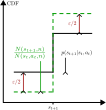
\includegraphics[scale=0.6]{figures/ch4/dkw_diagram.pdf}
                \caption[Bounding the empirical transition probabilities to the true transition probabilities.]{Bounding the empirical transition probabilities to the true transition probabilities. The true cdf is shown as a solid black line, the empirical cdf is shown as a dashed green line, and a worst case error of $\varepsilon/2$, using Theorem \ref{thrm:dkw_inequality}, is shown in red. The probability mass of $p(s_{t+1}|s_t,a_t)$ and empirical probability mass of $\frac{N(s_{t+1},n)}{N(s_t,a_t,n)}$ is also indicated to demonstrate how the constructed distribution gives Corollary \ref{cor:bound_transition_distribution}.}
                \label{fig:dkw_diag}
            \end{figure}
            %
            \begin{corollary} \label{cor:bound_transition_distribution}
                Consider any Boltzmann MCTS process. For all $(s_t,a_t)\in\cl{S}\times\cl{A}$ and for all $\varepsilon >0$ we have:
                \begin{align}
                    \Pr\left(\max_{s_{t+1}\in\suc{s_t}{a_t}}\left| \frac{N(s_{t+1},n)}{N(s_t,a_t,n)} - p(s_{t+1}|s_t,a_t) \right| > \varepsilon \right) \leq 2 \exp\left(-\frac{1}{2}\varepsilon^2 N(s_t,a_t) \right).
                \end{align}
            \end{corollary}
            \begin{proofoutline}
                By considering some arbitrary ordering over the successor states in $\suc{s_t}{a_t}$ and applying Theorem \ref{thrm:dkw_inequality}, replacing $\varepsilon$ by $\varepsilon/2$, the result follows.

                To see why the factor of $1/2$ is needed, consider Figure \ref{fig:dkw_diag}. Because the distribution is discrete, the cumulative distribution function is a (piecewise constant) step function. As Theorem \ref{thrm:dkw_inequality} bounds the maximum difference between the empirical and true cumulative distribution functions, the factor of $1/2$ is needed to account for the error before and after each $s_{t+1}$ in the worst case.
            \end{proofoutline}



        \todo{<end> dump (stuff put in main text)}

            


        Now that Corollary \ref{cor:bound_transition_distribution} can be used to bound  the empirical transition distribution to the true transition distribution,  a general purpose concentration inequality for Q-values can be proved for use in later proofs.

        \begin{lemma} \label{lem:stochastic_step}
            Consider any Boltzmann MCTS process, and some state action pair $(s_t,a_t)\in\cl{S}\times\cl{A}$. Let $\dot{V}^{N(s,n)}(s):\cl{S}\rightarrow \bb{R}$, $\dot{V}^*(s):\cl{S}\rightarrow \bb{R}$ be some estimated and optimal value functions respectively and suppose that for all $s_{t+1}\in\suc{s_t}{a_t}$ that there is some $C_{s_{t+1}}, k_{s_{t+1}}>0$ such that for all $\varepsilon_0 >0$:
            \begin{align}
                \Pr\left(\left| \dot{V}^{N(s_{t+1})}(s_{t+1}) - \dot{V}^*(s_{t+1}) \right| > \varepsilon_0 \right) \leq C_{s_{t+1}}\exp(-k_{s_{t+1}}\varepsilon_0^2 N(s')).
            \end{align}
            
            If the optimal and estimated Q-values are defined as follows: 
            \begin{align}
                \dot{Q}^*(s,a)&=R(s,a)+\bb{E}_{s'\sim p(\cdot|s,a)}\left[\dot{V}^*(s')\right], \\
                \dot{Q}^{N(s,a,n)}(s,a)&=R(s,a)+\sum_{s'\in\suc{s}{a}} \left[
                    \frac{N(s',n)}{N(s,a,n)} \dot{V}^{N(s',n)}(s')\right].
            \end{align}
            
            Then there exists some $C,k>0$, for all $\varepsilon>0$ such that:
            \begin{align}
                \Pr\left(\left| \dot{Q}^{N(s,a,n)}(s,a) - \dot{Q}^*(s,a) \right| > \varepsilon \right) \leq C\exp(-k\varepsilon^2 N(s,a,n)).
            \end{align}
        \end{lemma}

        \begin{proof}
            By the assumed bounds, Lemma \ref{lem:union_bound} and Lemma \ref{lem:s_to_sa}, there is some $C_1,k_1>0$, such that for any $\varepsilon_1 >0$:
            \begin{align}
                \Pr\left(\forall s_{t+1}. \left|\dot{V}^{N(s_{t+1})}(s_{t+1})-\dot{V}^*(s_{t+1}) \right| \leq \varepsilon_1 \right) > 1-C_1\exp(-k_1\varepsilon_1^2 N(s_t,a_t,n)). \label{local:one}
            \end{align}

            And recall that for any $p(s_{t+1}|s_t,a_t) > \varepsilon_2>0$, using Corollary \ref{cor:bound_transition_distribution} that:
            \begin{align}
                \Pr\left(\max_{s_{t+1}\in\suc{s_t}{a_t}} 
                    \left| \frac{N(s_{t+1},n)}{N(s_t,a_t,n)} - p(s_{t+1}|s_t,a_t) \right| 
                    \leq \varepsilon_2 \right) 
                        > 1 - 2 \exp\left(-\frac{1}{2}\varepsilon_2^2 N(s_t,a_t,n) \right). \label{local:two}
            \end{align}
            
            If the events in Inequalities (\ref{local:one}) and (\ref{local:two}) hold, then the following inequalities must also hold:
            \begin{align}
                \dot{V}^*(s_{t+1})- \varepsilon_1 
                    &\leq \dot{V}^{N_n(s_{t+1},n)}(s_{t+1}) 
                    \leq \dot{V}^*(s_{t+1})+ \varepsilon_1 \\
                p(s_{t+1}|s_t,a_t) - \varepsilon_2 
                    &\leq \frac{N(s_{t+1},n)}{N(s_t,a_t,n)} 
                    \leq p(s_{t+1}|s_t,a_t) + \varepsilon_2.
            \end{align} 
            
            The upper bounds on $\dot{V}^{N_n(s_{t+1},n)}(s_{t+1})$ and $N(s_{t+1},n)/N(s_t,a_t,n)$ can be used to obtain an upper bound on $\dot{Q}^{N(s_t,a_t,n)}(s_t,a_t)$: 
            \begin{align}
                &\dot{Q}^{N(s_t,a_t,n)}(s_t,a_t) \\
                    =& R(s_t,a_t) 
                        + \sum_{s_{t+1}\in\suc{s_t}{a_t}}\frac{N(s_{t+1},n)}{N(s_t,a_t,n)} 
                            \dot{V}^{N(s_{t+1},n)}(s_{t+1}) \\
                    \leq& R(s_t,a_t) 
                        + \sum_{s_{t+1}\in\suc{s_t}{a_t}}(p(s_{t+1}|s_t,a_t)+\varepsilon_2)
                            (\dot{V}^*(s_{t+1})+\varepsilon_1) \\
                    =& R(s_t,a_t) 
                        + \bb{E}_{s_{t+1}\sim p(\cdot|s_t,a_t)}[\dot{V}^*(s_{t+1})] 
                        + \varepsilon_1 
                        + \varepsilon_2\sum_{s_{t+1}\in\suc{s_t}{a_t}} \dot{V}^*(s_{t+1}) 
                        + \varepsilon_1 \varepsilon_2 \\
                    \leq& R(s_t,a_t) 
                        + \bb{E}_{s_{t+1}\sim p(\cdot|s_t,a_t)}[\dot{V}^*(s_{t+1})] 
                        + \varepsilon_2\left|\sum_{s_{t+1}\in\suc{s_t}{a_t}} \dot{V}^*(s_{t+1})\right| 
                        + \varepsilon_1 + \varepsilon_1 \varepsilon_2 \\
                    =& \dot{Q}^*(s_t,a_t) 
                        + \varepsilon_2\left|\sum_{s_{t+1}\in\suc{s_t}{a_t}} \dot{V}^*(s_{t+1})\right| 
                        + \varepsilon_1 
                        + \varepsilon_1 \varepsilon_2.
            \end{align}
            
            Following the similar reasoning but using the lower bounds on $\dot{V}^{N_n(s_{t+1},n)}(s_{t+1})$ and $N(s_{t+1},n)/N(s_t,a_t,n)$ gives: \todo{There is some special cases when V is negative, having to use the other bound, but the upper and lower bound have a bit of leway which handles all four cases of using plus minus epsilon one and two.}
            \begin{align}
                \dot{Q}^{N(s_t,a_t,n)}(s_t,a_t) 
                    &\geq \dot{Q}^*(s_t,a_t) 
                        - \varepsilon_2\left|\sum_{s_{t+1}\in\suc{s_t}{a_t}} \dot{V}^*(s_{t+1})\right| 
                        - \varepsilon_1 
                        - \varepsilon_1 \varepsilon_2.
            \end{align}
            
            Now given an arbitrary $\varepsilon >0$, recalling that $\varepsilon_1,\varepsilon_2>0$ were arbitrary, set $\varepsilon_1 = \varepsilon/3$ and $\varepsilon_2 = \min(\varepsilon/3, \varepsilon/3|\sum_{s_{t+1}} \dot{V}^*(s_{t+1})|)$ to give:
            %
            \begin{align}
                \dot{Q}^*(s_t,a_t) - \varepsilon \leq \dot{Q}^{N(s_t,a_t,n)}(s_t,a_t) \leq \dot{Q}^*(s_t,a_t) + \varepsilon.
            \end{align}
            
            Using Lemma \ref{lem:union_bound} liberally, there is some $C_2,C_3,k_2,k_3>0$ such that:
            \begin{align}
                &\Pr\left(\left| \dot{Q}^{N(s_t,a_t,n)}(s_t,a_t) - \dot{Q}^*(s_t,a_t) \right| \leq \varepsilon \right) \\
                    >& \left(1-C_1\exp(-k_1\varepsilon_1^2 N(s_t,a_t,n))\right) 
                        \left(1-2\exp\left(-\frac{1}{2}\varepsilon_2^2 N(s_t,a_t,n) \right)\right) \\
                    =& \left(1-C_2\exp(-k_2 \varepsilon^2 N(s_t,a_t,n) \right) 
                        \cdot \left(1-C_3\exp(-k_3 \varepsilon^2 N(s_t,a_t,n)\right) \\
                    % =& 1 -C_2\exp(-k_2 \varepsilon^2 N(s_t,a_t,n)) -C_3\exp(-k_3 \varepsilon^2 N(s_t,a_t,n)) \notag \\
                    %     &+ C_2C_3\exp(-(k_2+k_3)\varepsilon^2 N(s_t,a_t,n) ) \\
                    >& 1 -C_2\exp(-k_2 \varepsilon^2 N(s_t,a_t,n)) -C_3\exp(-k_3 \varepsilon^2 N(s_t,a_t,n)).
            \end{align}
            
            Finally, by negating and setting $C=C_2+C_3$ and $k=\min(k_2,k_3)$ in Lemma \todo{ref} the result follows:
            \begin{align}
                    \Pr\left(\left| \dot{Q}^{N(s_t,a_t,n)}(s_t,a_t) - \dot{Q}^*(s_t,a_t) \right| > \varepsilon \right) \leq C\exp(-k\varepsilon^2 N(s_t,a_t,n)).
            \end{align}
        \end{proof}








    \subsection{MENTS Results} 
    \label{appsec:ments_results}

        This subsection provides results related to MENTS in the setting of that standard reinforcement learning objective. Concentration inequalities are given around the optimal soft values to start with, although this result is similar to soem of the results provided in \cite{ments} \todo{this is still provided to keep this thesis' proofs self contained. (although its not as we use lots of things like hoeffdings, and also use UCT style proofs prsumably later on.) We could say ``to keep the proofs compatible with the other results provided. Or we could just omit it and reference the MENTS paper...''} Afterwards, the concentration inequalities are combined with results about maximum entropy reinforcement learning \todo{ref the section where we did that} to provide bounds on the simple regret of MENTS, given constraints on the temperature.
        








        To prove the concentration inequality around the optimal soft values, start by showing an inductive step.

        
        \begin{lemma} \label{lem:ments_val_induction_step}
            Consider a MENTS process. Let $s_t\in\cl{S}$, with $1\leq t \leq H$ \todo{update for thtspp notation}. If for all $s_{t+1}\in\bigcup_{a\in\cl{A}}\suc{s_t}{a}$ there is some $C_{s_{t+1}},k_{s_{t+1}}>0$ for any $\varepsilon_{s_{t+1}}>0$:
            \begin{align}
                \Pr\left(\left| \mVments{N(s_{t+1},n)}(s_{t+1}) - V_{\sft}^*(s_{t+1}) \right| > \varepsilon_{s_{t+1}} \right) 
                    &\leq C_{s_{t+1}}\exp\left( -k_{s_{t+1}}\varepsilon_{s_{t+1}}^2 N(s_{t+1},n) \right), 
            \end{align}
            then there is some $C,k>0$, for any $\varepsilon>0$:
            \begin{align}
                \Pr\left(\left| \mVments{N(s_{t},n)}(s_t) - V_{\sft}^*(s_{t}) \right| > \varepsilon \right) 
                    &\leq C\exp\left( -k\varepsilon^2 N(s_{t},n) \right).
            \end{align}
        \end{lemma}
        
        \begin{proof}
            Given the assumptions and by Lemmas \ref{lem:stochastic_step}, \ref{lem:sa_to_s} and \ref{lem:union_bound}, there is some $C,k>0$ such that for any $\varepsilon>0$:
            \begin{align}
                \Pr\left(\forall a_t\in\cl{A}. \left|\mQments{N(s_t,a_t,n)}(s_t,a_t)-Q_{\sft}^*(s_t,a_t)\right|\leq \varepsilon\right) &> 1-C \exp(-k \varepsilon^2 N(s_t,n)).
            \end{align}
            
            So with probability at least $1-C \exp(-k \varepsilon^2 N(s_t,n))$, for any $a_t$, the following holds:
            \begin{align}
                Q_{\sft}^*(s_t,a_t) - \varepsilon \leq \mQments{N(s_t,a_t,n)}(s_t,a_t) \leq Q_{\sft}^*(s_t,a_t) + \varepsilon. 
            \end{align}
            
            Using the upper bound on $\mQments{N(s_t,a_t,n)}(s_t,a_t)$ in the soft backup equation for $\mVments{N(s_t,n)}(s_t)$ (Equation (\ref{appeq:soft_v_backup}) gives:
            \begin{align}
                \mVments{N(s_t,n)}(s_t) &= \alpha \log \sum_{a\in\cl{A}} 
                        \exp\left(\frac{\mQments{N(s_t,a_t,n)}(s_t,a_t)}{\alpha}\right) \\
                    &\leq \alpha \log \sum_{a\in\cl{A}} \exp\left(\frac{Q_{\sft}^*(s_t,a_t)+\varepsilon}{\alpha}\right) \\
                    &= \left[\alpha \log \sum_{a\in\cl{A}} \exp\left(\frac{Q_{\sft}^*(s_t,a_t)}{\alpha}\right)\right] 
                        + \varepsilon \\
                    &= V_{\sft}^*(s_t) + \varepsilon,
            \end{align}
            noting that the \textit{softmax} function monotonically increases in its arguments. Then with similar reasoning using the lower bound on $\mQments{N(s_t,a_t,n)}(s_t,a_t)$ gives:
            \begin{align}
                \mVments{N(s_t,n)}(s_t) \geq V_{\sft}^*(s_t) - \varepsilon,
            \end{align}
            and hence:
            \begin{align}
                |\mVments{N(s_t,n)}(s_t)-V_{\sft}^*(s_t)| \leq \varepsilon.
            \end{align}
            
            This therefore shows: \todo{some comment about how if A implies B then pr(B) more than pr(A)}
            \begin{align}
                \Pr\left(\left|\mVments{N(s_t,n)}(s_t)-V_{\sft}^*(s_t)\right| \leq \varepsilon_1\right) > 1-C \exp(-k \varepsilon^2 N(s_t,n)),
            \end{align}
            and negating probabilities gives the result.
        \end{proof}









            
        
        Then completing the induction gives the concentration inequalities desired for any state that MENTS might visit.
        \begin{theorem} \label{thrm:ments_val_converge}
            Consider a MENTS process, let $s_t\in\cl{S}$ then there is some $C,k>0$ for any $\varepsilon>0$:
            \begin{align}
                \Pr\left(\left| \mVments{N(s_{t},n)}(s_{t}) - V_{\sft}^*(s_{t}) \right| > \varepsilon \right) 
                    &\leq C\exp\left( -k\varepsilon^2 N(s_{t},n) \right).
            \end{align}
            Moreover, at the root node $s_0$:
            \begin{align}
                \Pr\left(\left| \mVments{N(s_{0},n)}(s_{0}) - V_{\sft}^*(s_{0}) \right| > \varepsilon \right) 
                    &\leq C\exp\left( -k\varepsilon^2 n \right). \label{local:three}
            \end{align}
            And hence $\mVments{N(s_{t},n)}(s_{t}) \rap V_{\sft}^*(s_{t})$.
        \end{theorem}
        \begin{proof}
            Consider that the result holds for $t=H+1$, because $\mVments{N(s_{H+1},n)}(s_{H+1})=V_{\sft}^*(s_{H+1})=0$. Therefore the result holds for any $t=0,...,H+1$ by induction using Lemma \ref{lem:ments_val_induction_step}. Noting that $N(s_0)=n$ gives (\ref{local:three}). \todo{To see the convergence in probability, let }$n\rightarrow\infty$. \todo{Double check the H stuf is consistent with the thtspp and MDP defns}
        \end{proof}










        Provided MENTS's temperature parameter is set small enough, such that the optimal standard and soft values lead to identical recommendation policies \todo{ref the max entropy proof of this}, then MENTS is consistent and the expected simple regret tends to zero exponentially. This is shown in the following lemma.
            
        \begin{lemma} \label{lem:ments_imm_simple_regret}
            Consider a MENTS process with $\alphaments<\Delta_{\cl{M}}/3H\log |\cl{A}|$. \todo{Make sure replaced alpha with alphaments in ments theorems} Let $s_t\in\cl{S}$, with $1\leq t \leq H$ then there is some $C',k'>0$ such that:
            \begin{align}
                \bb{E} \sreg(s_{t},\mpsiments{n}) &\leq C'\exp\left( -k' N(s_{t},n) \right).
            \end{align}
        \end{lemma}
        \begin{proof}
            \todo{Why cant we just replace this with, the values converge in probability from the previous result, and then use that it means the recommendation policy converges in probability, and then use that to say simple regret go zero? The case where it doesnt work is if there is suboptimal soft value which equals the optimal soft value (which has no entropy), in this case, becase we need the value ESTIMATES to converge, not the optimal values, we need the temperature to be a bit stricter. I think}

            Let $a^*$ be the optimal action with respect to the soft values, so $a^*=\argmax_{a\in\cl{A}} Q_{\sft}^*(s_t,a)$. Then by Lemma \ref{lem:soft_standard_consistent_order} $a^*$ must also be the optimal action for the standard Q-value function $a^*=\argmax_{a\in\cl{A}} Q^*(s_t,a)$. By Theorem \ref{thrm:ments_val_converge} and Lemmas \ref{lem:stochastic_step} and \ref{lem:sa_to_s} there exists $C_1,k_1>0$ such that for all $\varepsilon_1>0$: \todo{reword this paragraph, its a bit meh}
            \begin{align}
                \Pr\left(\forall a_t\in\cl{A} \left|\mQments{N(s_t,a_t,n)}(s_t,a_t)-Q_{\sft}^*(s_t,a_t)\right|\leq \varepsilon_1\right) &> 1-C_1 \exp(-k_1 \varepsilon_1^2 N(s_t,n)).
            \end{align}
            
            Setting $\varepsilon_1=\Delta_{\cl{M}}/3H\log |\cl{A}|$ then gives with probability at least $1-C_1 \exp(-k_2N(s_t,n))$ (where $k_2=k_1\left(\frac{\Delta_{\cl{M}}}{3H\log|\cl{A}|}\right)^2$) that for all actions $a_t\in\cl{A}$:
            \begin{align}
                Q_{\sft}^*(s_t,a_t) - \Delta_{\cl{M}}/3 \leq \mQments{N(s_t,a_t,n)}(s_t,a_t) \leq Q_{\sft}^*(s_t,a_t) + \Delta_{\cl{M}}/3.
            \end{align}
            
            And hence, with probability at least $1-C_1 \exp(-k_2N(s_t,n))$, for all $a\in\cl{A}-\{a^*\}$ we have:
            \begin{align}
                \mQments{N(s_t,a,n)}(s_t,a)
                    \leq& Q_{\sft}^*(s_t,a) + \Delta_{\cl{M}}/3 \\
                    \leq& Q^*(s_t,a) + \alpha H\log |\cl{A}| + \Delta_{\cl{M}}/3 \\
                    \leq& Q^*(s_t,a) + 2\Delta_{\cl{M}}/3 \\
                    \leq& Q^*(s_t,a^*) - \Delta_{\cl{M}}/3 \\
                    \leq& Q_{\sft}^*(s_t,a^*) - \Delta_{\cl{M}}/3 \\
                    \leq& \mQments{N(s_t,a^*,n)}(s_t,a^*). \label{local:nine}
            \end{align}
            
            Where in the above, the first line holds from the upper bound on $\mQments{N(s_t,a_t,n)}(s_t,a_t)$; The second holds from maximising the standard return and entropy portions of the soft value separately (recall Inequality (\ref{appeq:softdiv}) in Lemma \ref{lem:soft_standard_consistent_order}); The third holds from the assumption on $\alpha$; The fourth holds from the definition of $\Delta_{\cl{M}}$ (also see Inequality (\ref{appeq:delta_diff})); The fifth holds from the optimal soft value being greater than the optimal standard value (Lemma \ref{lem:soft_geq_standard}); And the final line holds by using the lower bound on $\mQments{N(s_t,a_t,n)}(s_t,a_t)$ given above with $a_t=a^*$. 
            
            Negating the probability that (\ref{local:nine}) holds gives:
            \begin{align}
                \Pr\left(\exists a_t\in\cl{A}-\{a^*\}.\left( 
                    \mQments{N(s_t,a)}(s_t,a) > \mQments{N(s_t,a^*,n)}(s_t,a^*)\right)\right)
                    \leq C_1 \exp(-k_2N(s_t)).
            \end{align}
            
            The expected immediate regret can be bounded as follows:
            \begin{align}
                & \bb{E}\ireg(s_t,\mpsiments{n})  \\
                    =& \sum_{a\in\cl{A}-\{a^*\}} 
                        \left(V^*(s_t)-Q^*(s_t,a)\right) \Pr\left(\mpsiments{n}(s_t) =a \right) \\
                    =& \sum_{a\in\cl{A}-\{a^*\}} 
                        \left(V^*(s_t)-Q^*(s_t,a)\right) \Pr\left(a = \argmax_{a'} \mQments{N(s_t,a',n)}(s_t,a') \right) \\
                    \leq& \sum_{a\in\cl{A}-\{a^*\}} 
                        \left(V^*(s_t)-Q^*(s_t,a)\right) \Pr\left(\mQments{N(s_t,a,n)}(s_t,a) > \mQments{N(s_t,a^*,n)}(s_t,a^*)  \right) \\
                    \leq&  \sum_{a\in\cl{A}-\{a^*\}} 
                        \left(V^*(s_t)-Q^*(s_t,a)\right) C_1 \exp(-k_2N(s_t,n)),
            \end{align}
            where $k'=k_2$ and $C'=C_1\sum_{a\in\cl{A}-\{a^*\}} \left(V^*(s_t)-Q^*(s_t,a)\right)$. Finally, using \todo{ref lemma} gives the result.
        \end{proof}









        
        In consequence to Lemma \ref{lem:ments_imm_simple_regret}, provided the sufficient conditions are met, MENTS is consistent and will converge to a simple regret of zero.
        \begin{theorem} \label{thrm:ments_simple_regret_converge}
            Consider a MENTS process with $\alphaments<\Delta_{\cl{M}}/3H\log |\cl{A}|$.\todo{H consistent with thtspp}  Let $s_t\in\cl{S}$, with $1\leq t \leq H$ \todo{H consistent with thtspp} then there is some $C',k'>0$ such that:
            \begin{align}
                \bb{E} \sreg(s_{t},\mpsiments{n}) &\leq C'\exp\left( -k' N(s_{t},n) \right).
            \end{align}
            And specifically, at the root node $s_0$:
            \begin{align}
                \bb{E} \sreg(s_{0},\mpsiments{n}) &\leq C'\exp\left( -k'n) \right).
            \end{align}
        \end{theorem}
        \begin{proof}
            This theorem holds as a consequence of Corollary \ref{cor:imm_to_full_simple_regret} and Lemma \ref{lem:ments_imm_simple_regret}, and noting that at the root node $N(s_0,n)=n$.
        \end{proof}









        \todo{this was a theorem in the main neurips paper. Need to decide how writing this up, so this may go}
        \todo{We} have now shown Theorem \ref{thrm:ments}:
        \begin{customthm}{3.2} 
            For any MDP $\cl{M}$, after running $n$ trials of the MENTS algorithm with $\alphaments \leq \Delta_{\cl{M}}/3H\log|\cl{A}|$, \todo{H consistent with thtspp} there exists constants $C,k>0$ such that: $\bb{E}[\sreg(s_0,\psi^n_{\textnormal{MENTS}})] \leq C\exp(-kn)$, where $\Delta_{\cl{M}}=\min \{Q^*(s,a,t)-Q^*(s,a',t)\vert Q^*(s,a,t) \neq Q^*(s,a',t),s\in\cl{S}, a,a'\in\cl{A},t\in\bb{N}\}$.
        \end{customthm}
        \begin{proof}
            This is part of Theorem \ref{thrm:ments_simple_regret_converge}.
        \end{proof}






    \subsection{DENTS (and BTS) Results} 
    \label{appsec:dents_proofs}

        \todo{This is mostly the exponential bound stuff, so can also probably be appendix stuff}

        This subsection provides theoretical results that give exponential convergence of DENTS value estimates and simple regret. \todo{Some note on no constraints necessary on the parameters of DENTS?} 







        \begin{lemma} \label{lem:dents_val_induction_step}
            \todo{maybe should do directly from the Q values? Also same for the ments one?}
            Consider a DENTS process. Let $s_t\in\cl{S}$, with $1\leq t \leq H$. \todo{make H consistent with thtspp} If for all $s_{t+1}\in\bigcup_{a\in\cl{A}}\suc{s_t}{a}$ there is some $C_{s_{t+1}},k_{s_{t+1}}>0$ such that for any $\varepsilon_{s_{t+1}}>0$:
            \begin{align}
                \Pr\left(\left| \mVdents{N(s_{t+1},n)}(s_{t+1}) - V^*(s_{t+1}) \right| > \varepsilon_{s_{t+1}} \right) 
                    &\leq C_{s_{t+1}}\exp\left( -k_{s_{t+1}}\varepsilon_{s_{t+1}}^2 N(s_{t+1},n) \right), 
            \end{align}
            then there is some $C,k>0$, for any $\varepsilon>0$:
            \begin{align}
                \Pr\left(\left| \mVdents{N(s_{t},n)}(s_{t}) - V^*(s_t) \right| > \varepsilon \right) 
                    &\leq C\exp\left( -k\varepsilon^2 N(s_{t},n) \right).
            \end{align}
        \end{lemma}
        \begin{proof}
            Given the assumptions and by Lemmas \ref{lem:stochastic_step}, \ref{lem:union_bound} and \ref{lem:sa_to_s}, for some $C,k>0$ and for any $\varepsilon_1>0$:
            \begin{align}
                \Pr\left(\forall a_t\in\cl{A}. \left|\mQdents{N(s_t,a_t,n)}(s_t,a_t)-Q^*(s_t,a_t)\right|
                    \leq \varepsilon_1\right) &> 1-C \exp(-k \varepsilon_1^2 N(s_t)).
            \end{align}
            
            Let $\varepsilon >0$, and set $\varepsilon_1 = \min(\varepsilon,\Delta_{\cl{M}}/2)$. So with probability at least $1-C_1 \exp(-k_1 \varepsilon_1^2 N(s_t,n))$ for any $a_t$ it must be that:
            \begin{align}
                Q^*(s_t,a_t) - \varepsilon_1 \leq \mQdents{N(s_t,a_t,n)}(s_t,a_t) &\leq Q^*(s_t,a_t) + \varepsilon_1. 
                    \label{local:ten}
            \end{align}
            
            Let $a^*=\max_{a\in\cl{A}} Q^*(s_t,a)$. Using $\varepsilon_1 \leq \Delta_{\cl{M}}/2$ in (\ref{local:ten}), then for any $a\in\cl{A}-\{ a^*\}$:
            \begin{align}
                \mQdents{N(s_t,a,n)}(s_t,a) \leq& Q^*(s_t,a) + \Delta_{\cl{M}}/2 \\
                    \leq& Q^*(s_t,a^*) - \Delta_{\cl{M}}/2 \\
                    \leq& \mQdents{N(s_t,a^*,n)}(s_t,a^*),
            \end{align}
            and hence $\argmax_{a\in\cl{A}} \mQdents{N(s_t,a,n)}(s_t,a) = a^*$. As a consequence:
            \begin{align}
                \mVdents{N(s_t,n)}(s_t) &= \max_a \mQdents{N(s_t,a,n)}(s_t,a) = \mQdents{N(s_t,a^*,n)}(s_t,a^*). 
                    \label{local:editing_one}
            \end{align}
            
            Then using (\ref{local:ten}) with $a_t=a^*$ (noting $V^*(s_t)=Q^*(s_t,a^*)$), using (\ref{local:editing_one}) and using $\varepsilon_1 \leq \varepsilon$ gives:
            \begin{align}
                V^*(s_t) - \varepsilon
                    \leq& V^*(s_t) - \varepsilon_1 \\
                    \leq& \mVdents{N(s_t,n)}(s_t) \\
                    \leq& V^*(s_t) + \varepsilon_1 \\
                    \leq& V^*(s_t) + \varepsilon. 
            \end{align}
            
            Hence:
            \begin{align}
                \Pr\left(\left|\mVdents{N(s_t,n)}(s_t)-V^*(s_t)\right| > \varepsilon\right) 
                    &\leq C \exp(-k \varepsilon_1^2 N(s_t,n)) \\
                    &\leq C \exp(-k \varepsilon^2 N(s_t,n)),
            \end{align}
            which is the result.
        \end{proof}














        Similarly to the MENTS section, Lemma \ref{lem:dents_val_induction_step} provides an inductive step, which is used in Theorem \ref{thrm:dents_val_converge} to show concentration inequalities at all states that DENTS visits.
            
        \begin{theorem} \label{thrm:dents_val_converge}
            Consider a DENTS process, let $s_t\in\cl{S}$ then there is some $C,k>0$ for any $\varepsilon>0$:
            \begin{align}
                \Pr\left(\left| \mVdents{N(s_{t},n)}(s_t) - V^*(s_{t}) \right| > \varepsilon \right) 
                    &\leq C\exp\left( -k\varepsilon^2 N(s_{t},n) \right).
            \end{align}
            Moreover, at the root node $s_0$:
            \begin{align}
                \Pr\left(\left| \mVdents{N(s_{0},n)}(s_0) - V^*(s_0) \right| > \varepsilon \right) 
                    &\leq C\exp\left( -k\varepsilon^2 n \right). \label{local:four}
            \end{align}
        \end{theorem}
        \begin{proof}
            The result holds for $t=H+1$ \todo{consistent with thtspp. SHOULD JUST CTRL-F THIS and sort all of these out at once.} because $\mVdents{N(s_{H+1})}(s_{H+1})=V^*(s_{H+1})=0$. \todo{might be an off by one error here dep on how defined H, check over this whole paragraph.} Hence the result holds for all $t=1,...,H+1$ by induction using Lemma \ref{lem:dents_val_induction_step}. Noting that $N(s_0)=n$ gives (\ref{local:four}).
        \end{proof}









        \todo{is this just repeated? Can we merge two of the proofs?}

        Again, the concentration inequalities are used to show that the simple regret tends to zero exponentially, and therefore that DENTS will be exponentially likely in the number of visits to recommend the optimal standard action at every node.
            
        \begin{lemma} \label{lem:dents_imm_simple_regret}
            Consider a DENTS process. Let $s_t\in\cl{S}$, with $1\leq t \leq H$ \todo{defn with thtspp for H agen} then there is some $C',k'>0$ such that:
            \begin{align}
                \bb{E} \ireg(s_{t},\mpsidents{n}) &\leq C'\exp\left( -k' N(s_{t},n) \right).
            \end{align}
        \end{lemma}
        \begin{proof}
            Let $a^*$ be the locally optimal standard action, so $a^*=\argmax_{a\in\cl{A}} Q^*(s_t,a)$. By Theorem \ref{thrm:dents_val_converge} and Lemmas \ref{lem:stochastic_step} and \ref{lem:sa_to_s} there exists $C_1,k_1>0$ such that for all $\varepsilon_1>0$:
            \begin{align}
                \Pr\left(\forall a_t\in\cl{A}. \left|\mQdents{N(s_t,a_t,n)}(s_t,a_t)-Q^*(s_t,a_t)\right|\leq \varepsilon_1\right) &> 1-C_1 \exp(-k_1 \varepsilon_1^2 N(s_t,n)).
            \end{align}
            
            Setting $\varepsilon_1=\Delta_{\cl{M}}/2$ then gives with probability $1-C_1 \exp(-k_2N(s_t,n))$ (where $k_2=k_1\Delta_{\cl{M}}/2$) for all actions $a\in\cl{A}$ that:
            \begin{align}
                Q^*(s_t,a) - \Delta_{\cl{M}}/2 \leq \mQdents{N(s_t,a,n)}(s_t,a) \leq Q^*(s_t,a) + \Delta_{\cl{M}}/2.
            \end{align}
            
            And hence, with probability $1-C_1 \exp(-k_2N(s_t))$, for all $a_t\in\cl{A}-\{a^*\}$ it must be that:
            \begin{align}
                \mQdents{N(s_t,a,n)}(s_t,a_t)
                    \leq& Q^*(s_t,a_t) + \Delta_{\cl{M}}/2 \\
                    \leq& Q^*(s_t,a^*) - \Delta_{\cl{M}}/2 \\
                    \leq& \mQdents{N(s_t,a^*,n)}(s_t,a^*). \label{local:eleven}
            \end{align}
            
            Negating the probability of (\ref{local:eleven}) then gives:
            \begin{align}
                \Pr\left(\mQdents{N(s_t,a,n)}(s_t,a) > \mQdents{N(s_t,a^*,n)}(s_t,a^*)\right) \leq C_1 \exp(-k_2N(s_t,n))
            \end{align}
            
            Finally, the bound on the expected immediate regret follows:
            \begin{align}
                & \bb{E}\ireg(s_t,\mpsidents{n})  \\
                    =& \sum_{a\in\cl{A}-\{a^*\}} 
                        \left(V^*(s_t)-Q^*(s_t,a)\right) \Pr\left(\mpsidents{n}(s_t) =a \right) \\
                    =& \sum_{a\in\cl{A}-\{a^*\}} 
                        \left(V^*(s_t)-Q^*(s_t,a)\right) \Pr\left(a = \argmax_{a'} \mQdents{N(s_t,a,n)}(s_t,a) \right) \\
                    \leq& \sum_{a\in\cl{A}-\{a^*\}} 
                        \left(V^*(s_t)-Q^*(s_t,a)\right) 
                        \Pr\left(\mQdents{N(s_t,a,n)}(s_t,a) > \mQdents{N(s_t,a^*,n)}(s_t,a^*)  \right) \\
                    \leq&  \sum_{a\in\cl{A}-\{a^*\}} 
                        \left(V^*(s_t)-Q^*(s_t,a)\right) C_1 \exp(-k_2N(s_t,n)),
            \end{align}
            and setting $k'=k_2$ and $C'=C_1\sum_{a\in\cl{A}-\{a^*\}} \left(V^*(s_t)-Q^*(s_t,a)\right)$ gives the result.
        \end{proof}












        Again similarly to before, by using Lemma \ref{lem:dents_imm_simple_regret}, the bound on the immediate simple regret can be converted to a bound on the simple regret.
            
        \begin{theorem} \label{thrm:dents_simple_regret_converge}
            Consider a DENTS process. Let $s_t\in\cl{S}$, with $1\leq t \leq H$ \todo{thtspp consistent agen} then there is some $C',k'>0$ such that:
            \begin{align}
                \bb{E} \sreg(s_{t},\mpsidents{n}) &\leq C'\exp\left( -k' N(s_{t},n) \right).
            \end{align}
            
            Moreover, at the root node $s_0$:
            \begin{align}
                \bb{E} \sreg(s_{0},\mpsidents{n}) &\leq C'\exp\left( -k'n \right). \label{local:five}
            \end{align}
        \end{theorem}
        \begin{proof}
            Theorem holds as a consequence of Corollary \ref{cor:imm_to_full_simple_regret} and Lemma \ref{lem:dents_imm_simple_regret}. To arrive at (\ref{local:five}) note that $N(s_0,n)=n$.
        \end{proof}














        Theorem \ref{thrm:dents} follows \todo{this was the neurips main paper theorem, changing how doing the main results bit} from the results that we have just shown.


        Finally, Theorem \ref{thrm:dents} hows as it is a subset of what has already been shown.
        \begin{customthm}{4.2}
            \todo{this was the neurips main paper theorem, only changed enough to get this compiling. Also need to change the results for correct conditions, dont think beta needs to be bounded actually}
            For any MDP $\cl{M}$, after running $n$ trials of the DENTS algorithm with a root node of $s_0$, if $\betadents$ is bounded above and $\betadents(m)\geq 0$ for all $m\in\bb{N}$, then there exists constants $C,k>0$ such that for all $\varepsilon>0$ it holds that
            $\bb{E}[\sreg(s_0,\mpsidents{n})] \leq C\exp(-kn)$, and also $\mVdents{N(s_0,n)}(s_0) \rap V^*(s_0)$ as $n\rightarrow\infty$.
        \end{customthm}
        \begin{proof}
            The simple regret bound follows immediately from Theorem \ref{thrm:dents_simple_regret_converge}. Using Theorem \ref{thrm:dents_val_converge} it holds that $\Pr\left(\left| \mVdents{N(s_{0},n)}(s_0) - V^*(s_0) \right| > \varepsilon \right) \leq C\exp\left( -k\varepsilon^2 n \right) \rightarrow 0$ as $n\rightarrow \infty$, and hence $\mVdents{N(s_{0},n)}(s_0)$ converges in probability to $V^*(s_0)$.
        \end{proof}





        Finally, the BTS exponential convergence bound follows from it being a special case of DENTS.
        \todo{need to convert to new latex notation for thesis, so commented out below}
        % \begin{customthm}{4.1}
        %     For any MDP $\cl{M}$, after running $n$ trials of the BTS algorithm with a root node of $s_0$, there exists constants $C,k>0$ such that for all $\varepsilon>0$ we have $\bb{E}[\reg(s_0,\psi^n_{\textnormal{BTS}})] \leq C\exp(-kn)$, and also $\Vt{s_0}{N(s_0)} \rap V^*(s_0)$ as $n\rightarrow\infty$.
        % \end{customthm}
        % \begin{proof}
        %     Follows from setting $\beta(m)=0$ and using Theorem \ref{thrm:dents}.
        % \end{proof}


















